\documentclass[11pt,a4paper]{article}
\usepackage[left=2.3cm,top=2cm,right=2.3cm,bottom=2.0cm]{geometry}
\usepackage{geometry}
\usepackage{amsmath}
\usepackage{amssymb}
\usepackage{txfonts}
\usepackage{microtype}
\usepackage{epsfig}
\usepackage{graphicx}
\usepackage{moreverb}
\usepackage{hyperref}
\usepackage{listings}
\usepackage{xcolor}
\usepackage{textcomp}
\usepackage{makecell}
\usepackage{wasysym}
\definecolor{listinggray}{gray}{0.98}
\definecolor{lbcolor}{rgb}{0.98,0.98,0.98}
\lstset{
	backgroundcolor=\color{lbcolor},
	tabsize=4,
	rulecolor=,
	language=matlab,
    basicstyle=\scriptsize\ttfamily,
    upquote=true,
    aboveskip={1.5\baselineskip},
    columns=fixed,
    showstringspaces=false,
    extendedchars=true,
    breaklines=true,
    prebreak = \raisebox{0ex}[0ex][0ex]{\ensuremath{\hookleftarrow}},
    frame=single,
    showtabs=false,
    showspaces=false,
    showstringspaces=false,
    identifierstyle=\ttfamily,
    keywordstyle=\color[rgb]{0,0,1},
    commentstyle=\color[rgb]{0.133,0.545,0.133},
    stringstyle=\color[rgb]{0.627,0.126,0.941},
}

\usepackage{tikz}
\usepackage{pgfplots} 
\usepackage{pgfgantt}
\usepackage{pdflscape}
\usepackage{subcaption}
\usepackage{adjustbox}
\usepackage{siunitx}
\pgfplotsset{compat=newest} 
\pgfplotsset{plot coordinates/math parser=false}
\usepackage{pdfpages}
\usepackage{placeins}
\usepackage{wrapfig}





\newlength\fwidth
\newlength\fheight
\pagestyle{myheadings}

\pgfplotsset{every axis/.append style={
        scaled y ticks = false, 
        scaled x ticks = false, 
        y tick label style={/pgf/number format/.cd, fixed, fixed zerofill,
                            int detect,1000 sep={\;},precision=3},
        x tick label style={/pgf/number format/.cd, fixed, fixed zerofill,
                            int detect, 1000 sep={},precision=3}
    }
}

\usepackage{eso-pic}
\usepackage{ifthen}

\usepackage[nottoc]{tocbibind}
\usepackage[backend=biber,style=numeric,sorting=none]{biblatex}
\addbibresource{bibben.bib}

\usepackage{float}
\usepackage{subcaption}
\usepackage{gensymb}
\usepackage{siunitx}
\usepackage{enumitem}

\title{Project 3: Approximate Bayesian Computation}
\author{
  Kevin Andersson\\
  \texttt{kevinan@student.chalmers.se}
  \and
   Eric Lindgren\\
  \texttt{ericlin@chalmers.se}
}

\markright{Kevin Andersson and Eric Lindgren, Group 7}

\begin{document}

\maketitle

\pagenumbering{gobble}% Remove page numbers (and reset to 1)
% \newpage
\pagenumbering{arabic}% Arabic page numbers (and reset to 1)
\setcounter{page}{1}
\section{Introduction and Background}



\section{Methodology}

% BEskriv modellen här - kanske plotta några simulerade distributioner? Men ha inte med det i resultatet, endast NN och ABC i resultat.

\subsection[Task 1]{Neural network as a generator of prospective samples}
\label{sec:method_NN}
One issue with ABC is that convergence can be slow \cite{rasmusbaath}. In order to remedy this, we developed a neural network to generate candidates for the parameter $\alpha$ and the latent parameter $s$, given an input distribution from the simulator. By training the network, the hope is then that the prospective parameter samples generated by the network when fed with the observed distributions from the experiments will be more likely to be accepted by the ABC algorithm than drawing samples directly from the respective parameter priors, speeding up convergence. Hence, we generated a dataset consisting of 300000 distributions $\mathbf{X}$ from the simulator, each for different input parameters $y = (\alpha, s)$. The values for $\alpha$ and $s$ where drawn uniformly randomly in the respective intervals, $\alpha\in[0, 0.5]$ and $s\in[-0.25, 0.25]$. The neural network was trained to predict the parameters $y$, given the input distributions $\mathbf{X}$ with a 70\%/30\% training/validation split. Since the parameters $y$ are continuous, this corresponds to a regression problem. The network architecture consisted of two fully connected layers, of 32 and 2 units each, and no hidden layers. The input layer was activated using the ReLU function, with no activation being applied to the output layer in order to not constrain the output of the network (due to this being a regression problem). In order to monitor the training and the performance of the network, the loss function mean absolute error (MAE) was used. The network was implemented using Keras/Tensorflow.


\subsection[Task 4]{Approximate Bayesian Computation}
\label{sec:method_ABC}
% Nästan så man kanske vill flytta det här till ett teoriavsnitt? 
When performing Bayesian inference first you need some experimental data and then also a model connecting you unknown variable to the experiment by some theory. The goal is then to evaluate/sample the posterior
\begin{equation*}
    p(\theta|y_{obs}) \propto p(y_{obs}|\theta) p(\theta).
\end{equation*}
In some cases when the model is complicated it can be very hard our sometimes impossible to evaluate the likelihood, however there might be a way to, for a given set of parameters $\theta$, perform simulations. One can then evaluate the posterior by performing likelihood-free sampling. Likelihood-free sampling is based on rewriting the posterior as
\begin{equation*}
    p(\theta|y_{obs}) \propto \int d y \delta(y-y_{obs})p(y|\theta) p(\theta),
\end{equation*}
where $y_{obs}$ is some observed data. The posterior can thus be sampled by drawing $\theta^*$ from the prior $p(\theta)$, perform a simulation for $y^*  = f(\theta^*)$, and accept the sample if $y^* = y_{obs}$. This is an amazing result; we can sample the posterior even if we can't evaluate the likelihood analytically. But there might still be a crucial problem left tackle, namely that the requirement  $y^* = y_{obs}$ will give an acceptance ration equal to zero if the observed data is given by a continuous distribution of outcomes. This is also a problem the grows with the dimensionality in the observed data. The problem can be solved by Approximate Bayesian Calculation (ABC) which consists of replacing the delta function by 
\begin{equation*}
    p(\theta|y_{obs}) \propto \int d y \frac{1}{h}K\left(h^{-1}{||y - y_{obs}||}\right) p(y|\theta) p(\theta).
\end{equation*}
$K$ is the kernel satisfying $\int K(\xi)d\xi = 1$, $\int\xi K(\xi)d\xi = 0$ and $\int \xi^2K(\xi)d\xi < \infty$. $h$ is a parameter that governs the crudeness of the approximation and we see that if $h\mapsto 0$ ABC reduces to likelihood-free sampling. $||y - y_{obs}||$ is called a summary statistic and is a measure of similarity between the observed data and the simulated data. There exists many different summery statistics and the choice is up to the one performing the sampling; note however that one should be cautious about the choice since it can greatly effect the accuracy of the sampling and one should carefully investigate the approximation errors when doing approximate inference.

\subsection{Application of naive ABC to a toy problem}

In this report, we will apply ABC to a toy-problem consisting of a modified Galton board, as defined by equation \eqref{eq:galton}. The equation determines the probability of a bead hitting a peg on the Galton board to either turn left or right. The parameter $\alpha$ may thus be interpreted as the beads having a form of inertia, making the peg more likely to fall to the same side at the next peg as it did for the one before. The parameter $s$ is a bias, which makes the beads more likely to overall fall in a certain direction. 

\begin{equation}
    \label{eq:galton}
    P_{\pm} = 0.5 \pm \left(\alpha M + s \right)
\end{equation}

We will specifically perform inference on the $\alpha$-parameter. At hand we have a set of performed experiments all with the same but unknown $\alpha$, but all the experiments also has an independent unknown latent variable, the bias $s$. When performing ABC one would then normally draw both $\alpha$ and $s$ from a prior and accept the candidate $\alpha$ with a probability given by the kernel. However, since $s$ heavily affects the result of the experiment the acceptance ratio of the sampling would decrease dramatically. So to increase the acceptance ratio and thus speed up the convergence we use a neural network (NN) trained to determine $\alpha$ and $s$ from an experiment/simulation. We can thus instead of drawing $s$ from a prior draw it from a distribution defined by the NN prediction and its uncertainty. More precisely, we draw an $s^* \sim \mathcal{N}(s_m, \sigma_s)$, where $s_m$ is the prediction from the NN for $y_{obs}$ and $\sigma_s$ is the standard deviation in the predictive $s$ error for some simulated validation data. Our sampling of the posterior can then be summarized by the following algorithm. 
\begin{enumerate}
    \item $y_{obs} \mapsto \alpha_m, s_m$
    \item $s^* \sim \mathcal{N}(s_m, \sigma_s)$
    \item $\alpha^* \sim \pi(\alpha)$
    \item perform simulation $y = f(\alpha^*, s^*)$
    \item accept with probability $K(h^{-1}||y - y_{obs}||)$
    \item repeat 2-4
    \item repeat 1-5 for all $y_{obs}$
\end{enumerate}


When we now have our ABC algorithm in place we must decide on how to chose some hyper parameters to get the best performance in the sense of convergence speed and accuracy of the approximation. First we chose to use a Gaussian kernel 
\begin{equation*}
    K(\xi) = \frac{1}{\sqrt{2\pi \sigma^2}}\text{exp}\left(-\frac{\xi^2}{2\sigma^2}\right), \quad \sigma = \frac{1}{\sqrt{2\pi}}.
\end{equation*}
We chose the Gaussian since want the probability of acceptance to exponentially decrease when the similarity between the observed and simulated data decreases. We chose the $\sigma$ parameter so the kernel would have $K(0) = 1$, many other choices of $\sigma$ and the overall kernel could be tested but we restricted our study to the use of this kernel. The hyper parameter $h$ is tricky to chose and heavily depends on which summery statistic one uses (which will be presented below). Ideally one would like to chose $h$ small for the best approximation of the posterior, this on the other hand lead to low acceptance ratio and thus very slow convergence. Increasing $h$ would lead to faster convergence but a very crude approximation. There is however in the Bayesian sense a very elegant way to resolve this conflict, that is to perform several MCMC cycles where the posterior replaces the prior for the next cycle. One can then the drawn samples from the prior gets better and better lower $h$ for each cycle and thus get a better and better approximation for the posterior. There still exist a big question mark, that is how do we update $h$ and this is what the first part of the result will devoted to investigating. 

We know have come to the point where the we must decide upon a summery statistic. We need defina a way to measure a "distance" between experimental and simulated data. Since $y$ and $y_{obs}$ consist of a probability distribution over the slots in the Galton board a natural way to define the summary statistic is to take a distance measure between two probability distributions. For example one could use the Kulblack-leibler (KL) divergence, Wasserstein distance (WSD) our the energy distance (ED). Another summary statistic could be the ordinary L2 norm where each slot is regarded as a separate dimension. This is however usually not disarible measures since the large (32) dimensionallity the goal of a summary statistic is to reduce the dimensional to something describing all relevant information. A natural way to do this is to look at the mean and standard deviation of the distribution and for example take the diffrence of the mean for the experimental and simulated data as the summary statistic. We can from the model of the Galton board suspect that the standard deviation might be correlated with the value of $\alpha$, this might however not apply if $s$ is large or small and all bead ends up int either corner. Fortunately we have a very good way of reducing the dimensionality and keeping all relevant information namely doing a prediction with the neural network. So one very interesting summary statistic could be to take the difference between the predicted $\alpha$ for the observed and simulated data. To decide which one to use we tested all of them when performing several MCMC cycles with the obtained updating scheme of $h$ to find a converged posterior for all summary statistics. We could then evaluate their performance and decide upon which to use.

Finally we have thus specify all parts of the ABC algorithm up to the designer our describe how we evaluated them. We can thus perform a final sampling with the best updating scheme and summary statistic to obtain our posterior and then perform the inference for $\alpha$.


The nice thing with this algorithm from a Bayesian perspective is that it may be repeated, where the sampled posterior for $p(\alpha|y_{obs})$ replaces the prior $\pi(\alpha)$ for the next MCMC cycle. By repeating this procedure multiple times the confidence interval for the parameter $\alpha$ may be greatly reduced. This then naturally raises the question about the parameter $h$: when the cycle is repeated, the samples drawn from the prior $\pi(\alpha)$ gets repeatedly better, and thus an increasingly more restrictive $h$ may be used. 

% Skrev vidare på din del lite, tyckte det du hade skrivit var väldigt bra så tyckte det var snyggt att fortsätta så här. Feel free att ta bort det om du hade någon annan fortsättning i åtanke :)




\subsection{Improvements to our ABC implementation}

We now have a naive implementation of the ABC algorithm for the Galton board where have studied different summary statistics and the choice of $h$ for best performance. But as we will see in the result we still have a rather large confidence interval for the $\alpha$ parameter, and it does not decrease as the number of experiments increases. We thus have an improvement to the naive approach to lower the confidence interval. In the naive implementation we repeated the same algorithm for all observed $y_{obs}$ and added sampled $\alpha$'s. This is basically equivalent to evaluating the posterior for only one observed datum and then averaging the posterior for multiple observed data. Altough this average gives somwhat rubuster sampling against outliers in the data it does not decreas the confidence interval. So to use all the experiments we can assume them to be independent rewrite the posterior as
\begin{equation*}
    p(\theta|y_{obs}) \propto  \prod_i p(y_{obs,i}|\theta)\pi(\theta) = \prod_{i} \int d y_i \delta(y_i-y_{obs, i})p(y|\theta) p(\theta).
\end{equation*}
This would lead to an ABC algorithm where we have to replace all delta functions with kernels and evaluating the multidimensional integral. This would certainly be possible but we chose another approach. Instead of factorizing the likelihood we write the posterior like 
\begin{equation*}
    p(\theta|\hat{D}) = \int dD \delta(D - \hat{D}) p(D|\theta) \pi(\theta) = \int dD \frac{1}{h} K(h^{-1}||D - \hat{D}||) p(D|\theta) \pi(\theta).
\end{equation*}
Here $\hat{D}$ is the experimental data and $D$ is a simulated data set of the same size. So bye simulating a hole data set an compare to all observed data we use all information we have. So in this case we instead of defining a similarity measure between one experiment and one simulation we need to define a similarity measure between a experimental data set and a simulated one. With this interpretation the algorithm for sampling the posterior becomes


\begin{enumerate}
    \item $\alpha^* \sim \pi(\alpha)$
    \item $y_{obs,i} \mapsto \alpha_{m,i}, s_{m,i}$
    \item $s_i^* \sim \mathcal{N}(s_{m,i}, \sigma_s)$
    \item perform simulations $D = y_i = f(\alpha^*, s_i^*)$
    \item accept with probability $K(h^{-1}||D - \hat{D}||)$
    \item repeat 2-4
    \item repeat 1-5 for all $y_{obs}$
\end{enumerate}


One major thing that we glossed over in the previous section is how to handle $y_{obs}$ in the case when one has the results from N experiments, i.e. a dataset such that $\mathbf{y_{obs}} = \mathcal{D} = \left\{y_{obs,1}, y_{obs,2}, ..., y_{obs,N}\right\}$. In the earlier implementation the algorithm was simply repeated for all observed data, trying to accept different candidates $\alpha^*$ for each $y_{obs,i}$. However, since in this case the observed data all have the same value for the parameter $\alpha$, but different values for the latent variable $s$, one can instead see them as a dataset of $N$ datapoints which a candidate $\alpha^*$ would have be able to replicate well enough in order to be accepted. 

To fix the ideas, for our implementation specifically, we modify the algorithm as follows: Start with $N$ observed outcomes from the experiment $\mathcal{D} = \{y_{obs,i}\}_{i=1}^N$ and $M$ candidates $\{\alpha_j^*\}_{j=1}^M$. Use the NN to obtain estimates for the latent variables $\{s_{m,i}\}_{i=1}^N$, and draw a set of $\{s_i^* \sim \mathcal{N}(s_{m,i}, \sigma_s)\}_{i=1}^N$. Then, for each $\alpha_j^*$, perform $N$ simulations $\hat{y_i} = \texttt{simulation}(\alpha_j^*, s_i^*)$. A summary statistic $\mathcal{S}$ may then be applied to all pairs $\left\{(y_{obs,i}, \hat{y_i})\right\}_{i=1}^N$, $\mathcal{S}(\mathcal{D}, \mathbf{\hat{y}}) \mapsto x_j$. In other words, the information in the $N$ distributions is reduced to a single, scalar value of the summary statistic, $x_j$, which can be fed into the kernel to yield the probability of accepting the candidate $\alpha_j^*$: $p(\alpha_j^* \left. \vert \right. \mathcal{D} ) =  K(h^{-1}x_j)$. 



% This modified algorithm raises the threshold of acceptance for a certain candidate $\alpha^*$, which may thus yield a smaller CI for $\alpha$, but at the cost of possible having to consider many candidates $\alpha^*$ in order to obtain a well sampled posterior. Hence, implementing this algorithm may lead to a greatly increased computational cost compared to the naive way to handle multiple datapoints $y_{obs}$ as described in the previous section.

% Sen skriva om vår implementation här i detalj? Att vi valde NN som summary statistic, vilka settings vi körde etc?








% naive appoach 
    % - motivate the choice of h 
    % - motivate summary statistic 

% different amount of data

% \subsection{Approximate Bayesian Computation}
% study different kernals

% Kernels:
    % - Mean
    % - EUC
% More data
    % -
    
    
% Results
    % - (Kanske generella resultat)
    % 1. Undersöka effekt av kernels - ta upp alla
    % 2. Undersöka hanteringen av datan
    %
    
    
% Naive
    % Kernels
        %- Mean, EUC, KL
    % Data
% Advanced
    % Kernels
        % 
    % Data--




\section{Results and discussion}

In this section, we present and discuss our findings for using ABC to infer the parameter $\alpha$ in the modified Galton board model. We begin by discussing how to update $h$ between MCMC cycles, where we compare the inference results for using a fixed $h$ and when using an empirical scheme for updating $h$ of our own design. We then compare the results for when using different summary statistics in the naive implementation. Finally, we present the results for our improvements to the naive ABC algorithm, specifically for our implementation of considering observed data as a data set instead of individual data points. 

\subsection[Task 1]{Updating $h$ over multiple MCMC cycles in naive ABC}
\label{sec:result_h}

The empirically obtained updating scheme for $h$ that is used is given in equation \eqref{eq:emprical_h},

\begin{equation}
    \label{eq:emprical_h}
    h_{i+1} = \frac{h_i}{1+0.25\frac{\gamma_i}{\gamma_{i-1}}}.
\end{equation}
The goal of this updating scheme is to decrease $h$ at a rate that is governed by the change in acceptance ratio between cycles. We define the acceptance ratio to be the number of accepted $\alpha^*$ out of all proposed candidates. If the acceptance ratio decreases for cycle $i$ of MCMC as compared to the previous one, $\gamma_i>\gamma_{i-1}$, then $h$ will be decreased more than if $\gamma_i<\gamma_{i-1}$. Note that $h$ will never increase between cycles. Thus, $h$ will be decreased more if the acceptance ratio increases between cycles; this is because we expect the acceptance ratio to be artificially high for the early MCMC cycles, in which $h$ is too large. However, at some point, we expect that the obtained posterior, and thus the prior for the next cycle, converges towards the true posterior. When that happens, we desire an acceptance ratio that is close to one, since almost all of the candidates should be drawn from the true posterior. This scheme for updating $h$ does not reflect this behaviour, but the scheme can be extended by setting a minimum value for $h$. We opted for not doing this for simplicity, instead focusing on tuning the number of MCMC cycles.

\begin{figure}[ht]
    \centering
    \begin{subfigure}{.46\textwidth}
          \centering
          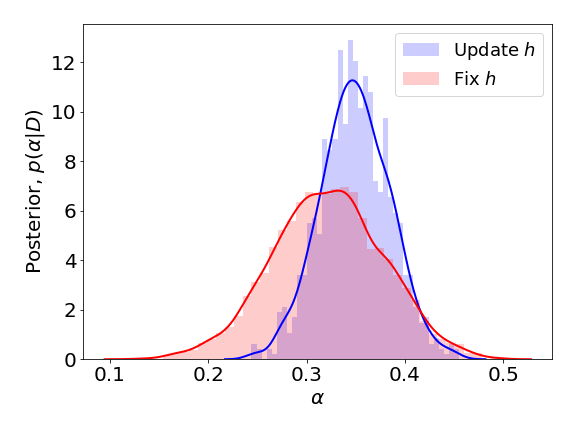
\includegraphics[width=1\textwidth]{figures/h_posterior.png}
          \caption{Posteriors for $\alpha$ after ten MCMC cycles} 
          \label{fig:h_posterior}
    \end{subfigure}%
    \begin{subfigure}{.46\textwidth}
          \centering
          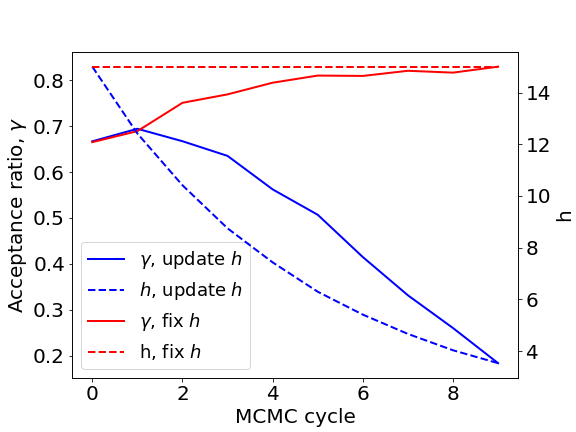
\includegraphics[width=1\textwidth]{figures/h_evolution.png}
          \caption{History over acceptance ratio and $h$}
    \label{fig:h_evolution}
    \end{subfigure}
    \caption{RMSE compared to the ground-truth PES as monitored during the training of the general-purpose GP, as well as predicted and ground-truth potential energy along the studied transition path.}
    \label{fig:h}
\end{figure}


The obtained posterior distributions after ten MCMC cycles with the Wasserstein distance, WSD, as a summary statistic and a uniform $\mathcal{U}(0, 0.5)$ initial prior for $\alpha$, either with a fixed value $h$ or with an $h$ that is updated for each cycle is given in figure \ref{fig:h_posterior}. The evolution of $h$ and the acceptance ratio for each of the two cases are given in figure \ref{fig:h_evolution}. We observe that the posterior for the case of updating $h$ is not as broad as when using a fixed $h$. Furthermore, studying the trace over the acceptance ratio in figure \ref{fig:h_evolution}, we see that the acceptance ratio decreases over the MCMC cycles when $h$ is decreased, as compared to the increasing acceptance ratio when $h$ is fixed. These results thus indicates that updating $h$ according to our scheme leads to a more restrictive acceptance of candidates for $\alpha$, which decreases the confidence interval. We will thus use this scheme for updating $h$ in the following sections.


\subsection[Task 1]{Comparison of summary statistics in naive ABC}
\label{sec:result_comp_sum_stat}

In this section we compare six different choices for six different summary statistics: Kullblack-Leibler divergence (KL), Wasserstein distance (WSD), energy distance (ED), the difference between the mean of the distributions (MEAN), the euclidian distance between the distributions (EUC) and using the neural network (NN). We are primarily interested in two aspects of these summary statistics. Firstly, do they capture the information necessary to infer $\alpha$? This can be seen in what value of $\alpha$ the respective posteriors converge to; if all summary statistics converge to the same $\alpha$, then they probably encode similar information. Secondly, we are interested in how the summary statistics affect the convergence speed. This can be seen from the size of the confidence interval (CI) after the same number of MCMC cycles. 

\begin{table}[h]
    \centering
    \caption{Obtained mean prediction for $\alpha$ together with a one standard deviation CI after ten MCMC cycles for the six different summary statistics.}
    \begin{tabular}{||c c c c c c||} 
         \hline
         KL & WSD & ED & EUC & MEAN & NN \\ [0.5ex] 
         \hline
         $0.361 \pm 0.027$ & $0.338 \pm 0.048$ & $0.330 \pm 0.057$ & $0.304 \pm 0.055$ & $0.210 \pm 0.069$ & $0.348 \pm 0.015$ \\ [0.5ex]
         \hline
    \end{tabular}
    \label{tab:sum_stat}
\end{table}

The mean and a confidence interval of one standard deviation for each of the summary statistics after ten MCMC cycles is given in table \ref{tab:sum_stat}. The empirical scheme for updating $h$ in equation \eqref{eq:emprical_h} was used, with the initial $h$ adjusted for each summary statistic. We observe that all summary statistics converge to roughly the same region, $\alpha \sim 0.3$, except for MEAN. This indicates that comparing the mean of the simulated and experimental distributions does not contain enough information on $\alpha$ for an accurate inference. As noted in the methodology, this could be due to $\alpha$ possibly affecting the spread of the distribution (and thus the standard deviance) rather than the mean. Comparing the remaining summary statistics, we note  that the one that yields the smallest confidence interval after ten MCMC cycles is the NN, which would indicate that using this summary statistic leads to the fastest convergence. This is perhaps not surprising, since the neural network is trained on this specific problem to extract as much information of the input distribution, i.e. summarize it, into it's prediction for the two parameters $\alpha$ and $s$. The use of the NN is thus a problem specific statistic, as compared to the others which are all general. This also introduces direct dependence of the result on the neural network, which is not the case when we only use it to generate proposals $\alpha^*$. Thus, if one is to use the neural network, one should be careful when training and evaluating the network so that its limitations and biases are known. We will use the NN as a summary statistic in the following sections, due to it outperforming all of our other candidates.


\subsection[Task 4]{Improved ABC -- }
\label{sec:result_ABC}

% TODO Lägg till modell från task 3

\printbibliography

\end{document}
